\section{Method}
\label{ch3:sec:method}

% !TEX root = ../main.tex
% !TEX spellcheck = en-US

\begin{figure}[b]
    \centering
    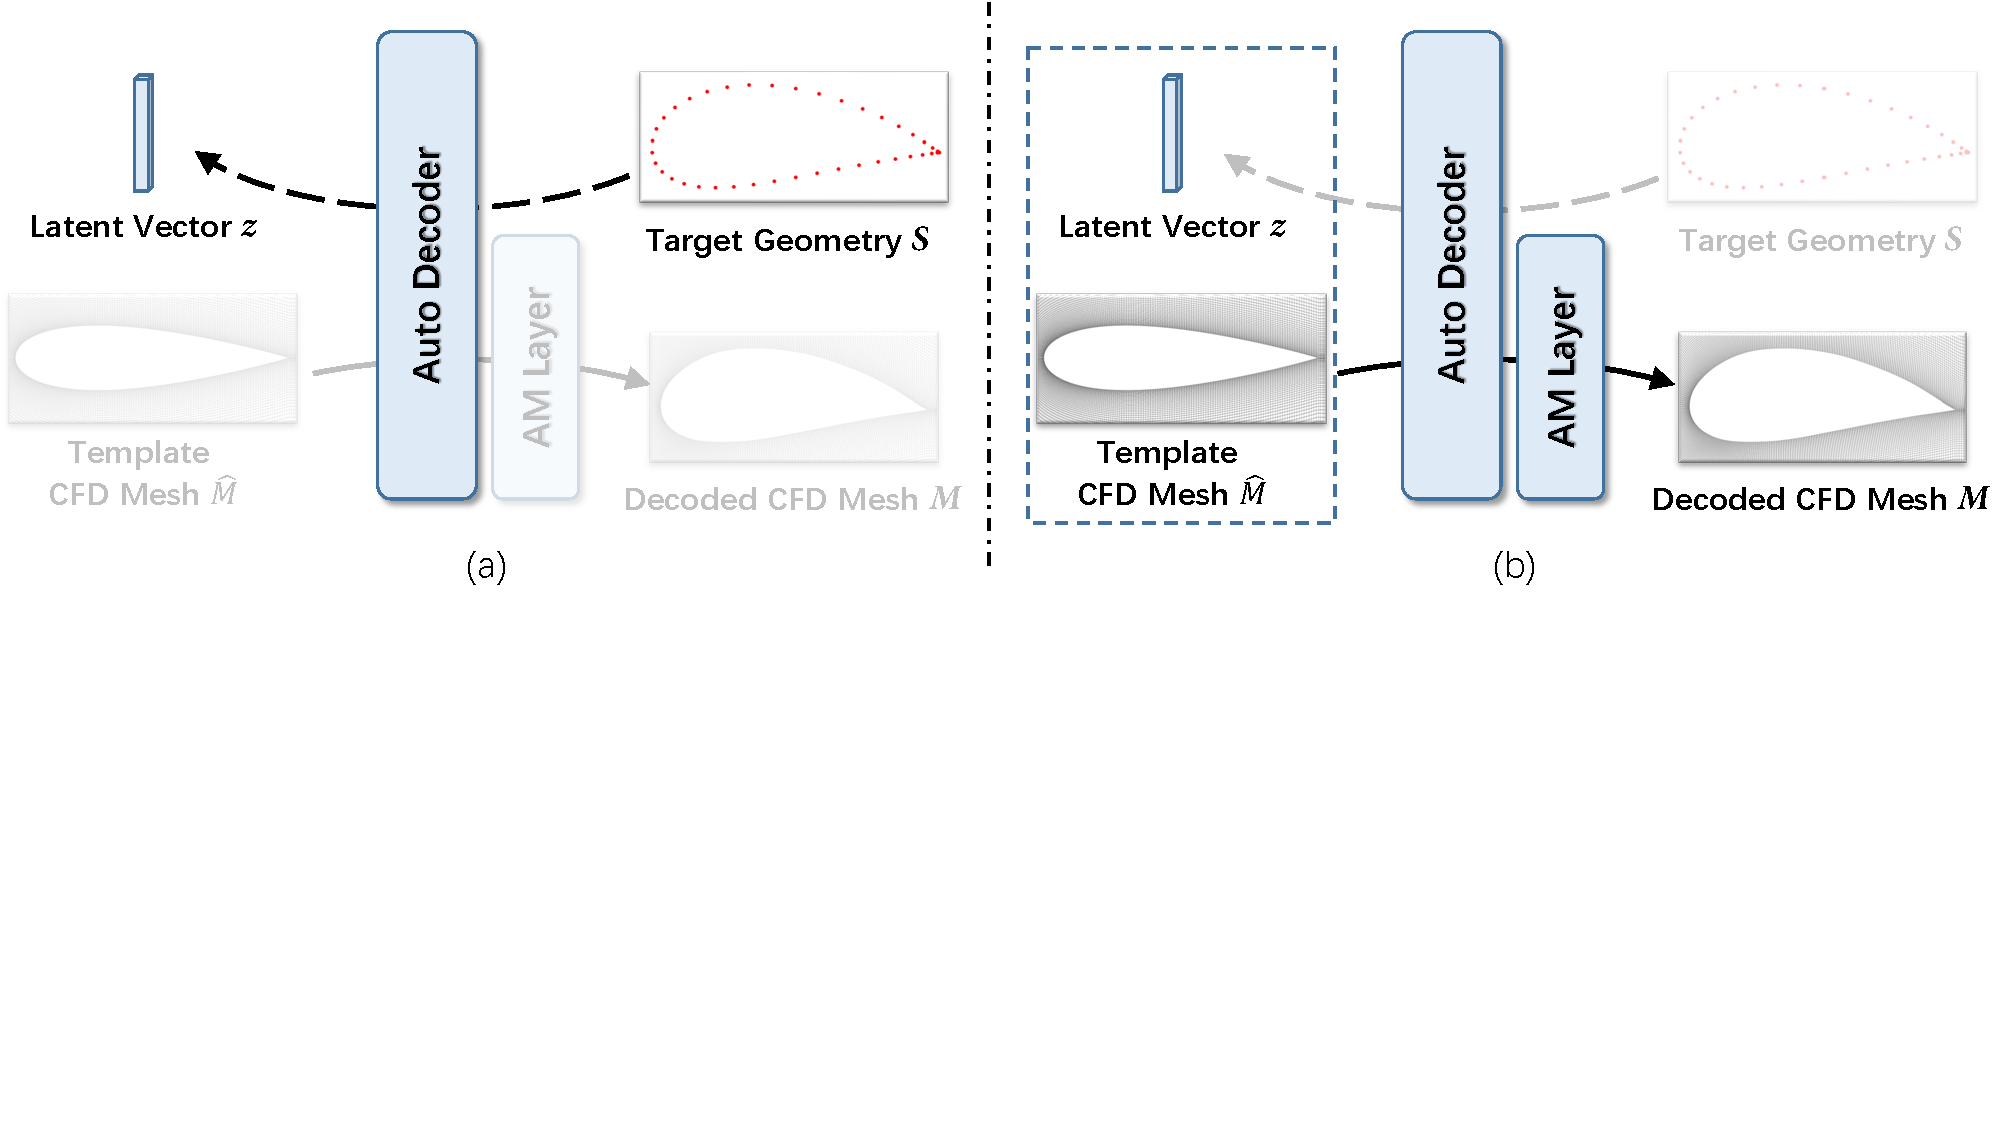
\includegraphics[width=0.97\linewidth]{chapter3/tex/figures/pipeline.pdf}
    \caption{\small Pipeline of the proposed model, including (a) the encoding step and (b) the decoding step.}
    \label{ch3:fig:arch}
\end{figure}


The proposed model is based on deep geometric learning to provide a flexible tool for mesh representation.
It is designed to encode a reference airfoil shape and then deform a fixed CFD mesh to reconstruct the geometry. In particular, only points sampled on the airfoil's surface are fed into the pipeline and an entire CFD mesh is generated after encoding and decoding the latent vector.
The pipeline is shown in Fig.\ref{ch3:fig:arch}.
In Section \ref{ch3:sec:Experiments}, demonstration is in a CFD context where the deformed mesh is employed to perform further CFD computations, including the optimization of the aerodynamic performances of a 2D airfoil.  In the remainder of this section, we first formalize this process in Section~\ref{ch3:sec:formal}, and then we describe the neural network and training details used to implement it. 

\subsection{Formalization}
\label{ch3:sec:formal}

\begin{figure}[!tb]
	\begin{center}
		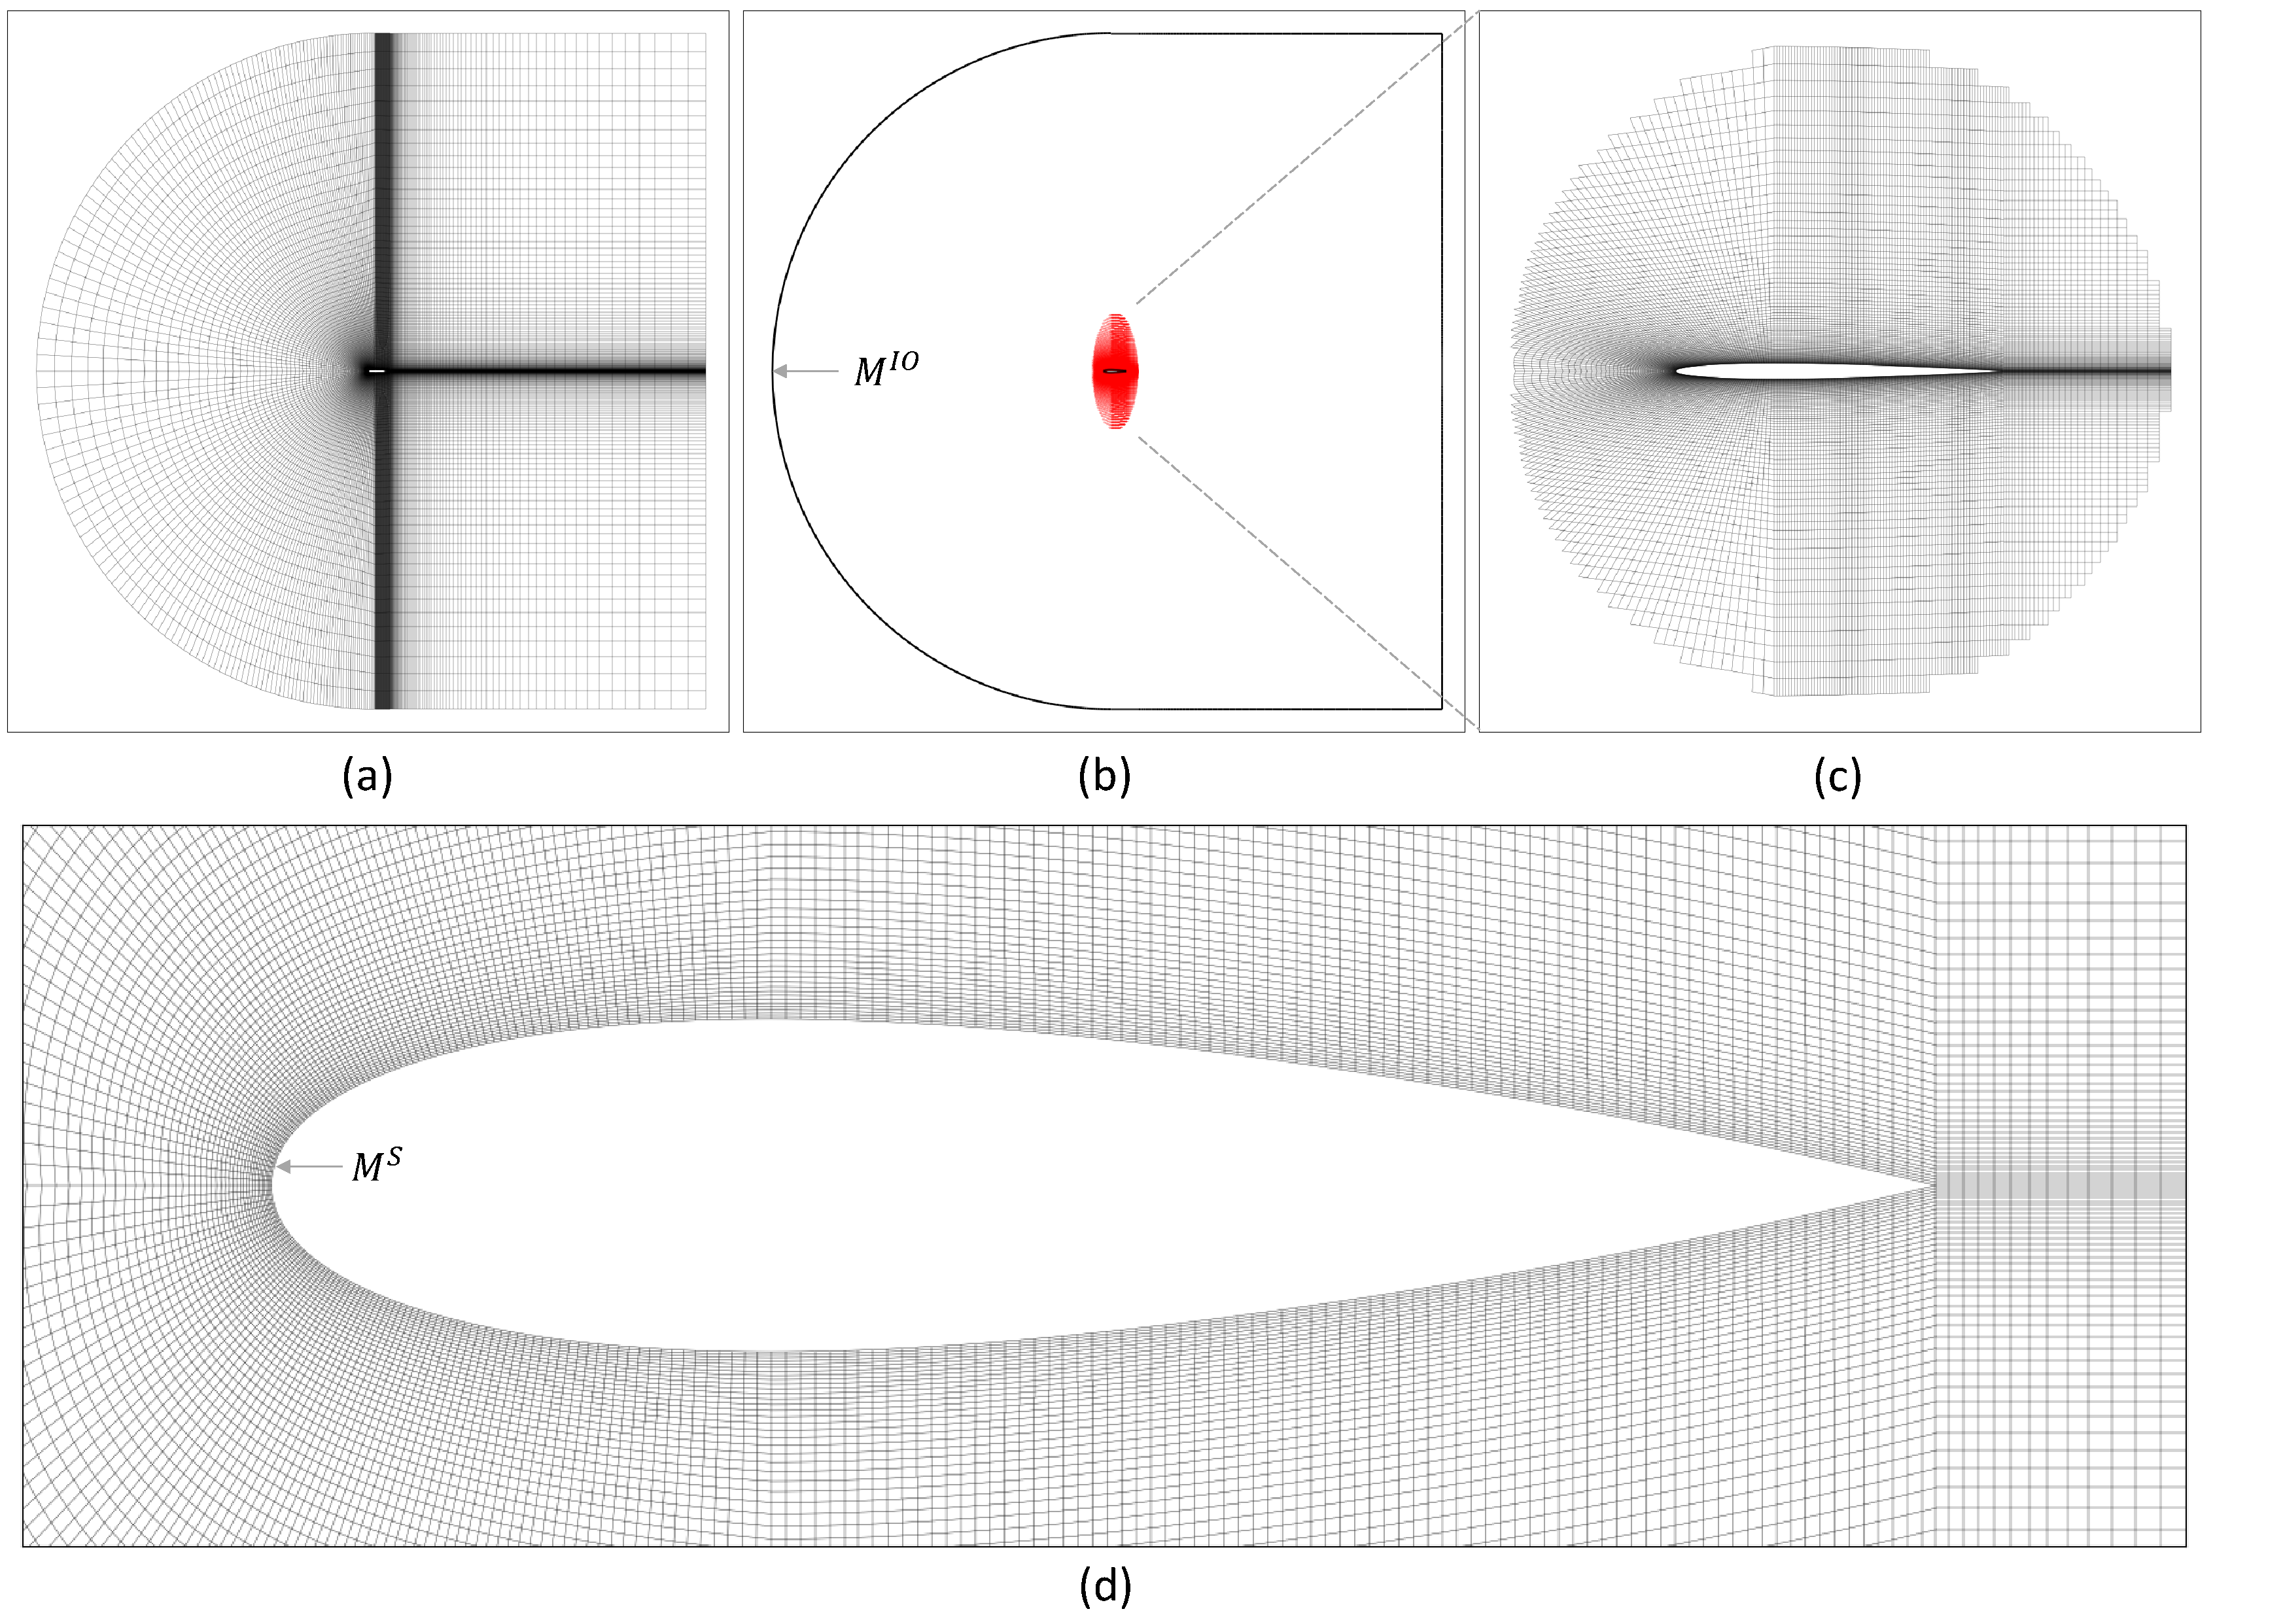
\includegraphics[width=1.01\linewidth]{chapter3/tex/figures/experiment/init_template_mesh_default.pdf}
	\end{center}
	\caption{ \small
		The default template mesh (TM-A) and its (a) overall mesh, (b) boundary, (c) deformation area and (d) surface.
	}
	\label{ch3:fig:exp_default_template}
\end{figure}

Consider a two dimensional airfoil shape represented by a CFD mesh $\hat{M}=\{\hat{V},\hat{E}\}$. The mesh contains $N$ 2D vertices $\hat{V}=\{\hat{\bv}_1, \hat{\bv}_2, ..., \hat{\bv}_N\}$, where $\hat{\bv}_i \in \mathbb{R}^2$, and edges $\hat{E}$ connecting its vertices. $N$ can be arbitrary. Let $\hat{V}^S$ and $\hat{E}^S$ be the subsets of vertices and edges in the surface mesh $\hat{M}^S$ that define the airfoil's profile, and $\hat{M}^{IO}$ be the inflow and outflow boundaries, also known as the inlet and outlet mesh. They define the computational boundary, as shown in Fig.~\ref{ch3:fig:exp_default_template}. A deformed mesh of the same topology can be represented as ${M}=\{\hat{V}+\Delta V,\hat{E}\}$, where $\Delta V$ is a set of translation vectors, one for each vertex. Note that the proposed framework is intended to encode and decode a geometry by mesh deformation so that the connectivity remains the same.

Let $D=2N$, $\bv$ be the $D$-vector obtained by stacking all the 2D coordinates of the $N$ vertices of $M$, and $\mathbf{\delta v}$ the vector of vertex translations represented by  $\Delta V$. This enables us to write that $\bv = \hat{\bv} +  \mathbf{\delta v}$, where $\hat{\bv}$ describes the vertices of $\hat{M}$. Finally, let $M(\bv)$ be the mesh with edges $\hat{E}$. Given these definitions, learning a low-dimensional representation of the mesh means finding a mapping parametrized by $\Theta$
%
\begin{align}
    g_{\Theta} : \mathbb{R}^d \rightarrow \mathbb{R}^D \; , \label{ch3:eq:map} \\
    \mathbf{\delta v} = g_{\Theta}(\bz; \hat{M}) \; , \nonumber
\end{align} 
%
where $d \ll D$, and $\bz\in \mathbb{R}^d$ is the so-called low-dimensional latent vector. $\Theta$ represents the weights that control the behavior of the deep neural network that implements $g$. 
We denote the decoded mesh deformation as $g_\Theta(\bz)$ when $\hat{M}$ is fixed in the following discussions for simplicity. 

The pipeline encodes and then decodes to fit a target airfoil represented by a geometry $S$, which is a set of surface sampling points.
No topology information is required in $S$, which removes the need for complicated data pre-processing and facilitate the use of various data formats. Despite $S$ being only an unstructured point cloud, the decoded output consists in a full computational mesh $M$ which is a smooth deformation of $\hat{M}$.

To learn the weights $\Theta$, we use an auto-decoding approach~\cite{ai.Tan1995,ai.Park2019c}. Given a set of $T$ training geometries that are only composed of sampled surface points, denoted $S_1,\ldots,S_T$, we seek
%
\begin{align}
\Theta^*,\bZ^* &=  \argmin_{\Theta,\bz_1,\ldots,\bz_T} \sum_{t=1}^T \cL(M(\hat{\bv} + g_{\Theta}(\bz_t)) , S_t) \; ,
\label{ch3:eq:autoenc}
\end{align}
%
where $\cL$ is a loss function that is small when $g_{\Theta}(\bz_t)$ yields a deformed mesh that is regular and whose profile defined by $\hat{V}^S$ and $\hat{E}^S$ is close to $S_t$ after deformation. Here, the optimal $\bz_t$ corresponds to a low-dimensional representation of the complete airfoil shape $S_t$.

At inference time, given a target airfoil profile $S$ and frozen weights $\Theta^*$, we solve
%
\begin{align}
\bz^* &=  \argmin_{\bz} \cL(M(\hat{\bv} + g_{\Theta^*}(\bz)) , S) \; .
\label{ch3:eq:autodec}
\end{align}
%
In other words, the latent vector $\bz$ parameterizes the possible profiles, and their corresponding computational mesh. We adjust this code to be as close as possible to the target $\bz^*$ so that the overall mesh $M$ corresponds to the target profile $S$. 

\subsection{Loss Function}
\label{ch3:sec:loss}

The mesh deformation pipeline relies on the latent code $\bz$ that provides a low-dimensional representation of the airfoil, and on the function $g_{\Theta^*}$ that returns the vector of vertex deformation $\mathbf{\delta v}$ of the mesh. They are learned by minimizing the loss function $\cL$ of  Eq.~\ref{ch3:eq:autoenc}. Given a decoded CFD mesh $M=M(\mathbf{\hat{v}} +g_{\theta}(\bz))$ and a target airfoil profile $S_t$, $\cL(M,S_t)$ of Eq.~\ref{ch3:eq:autoenc} should be small if, and only if, 
%
\begin{enumerate}

    \item the airfoil profile defined by $M$, namely $M^S$, is very similar to the target profile $S_t$,
    
    \item the computational mesh quality of $M$ is adequate for CFD simulations.
    
\end{enumerate}
%
Furthermore, unnecessary deformations should be penalized and latent space representations whose dimensionality is too high should be discouraged to guarantee $d \ll D$. Hence we write
%
\begin{equation}
    \cL = w_{dist}\cL_{dist} + w_{reg}\cL_{reg} + w_{dec} \cL_{dec} + w_{z} \cL_{z} \;,
    \label{ch3:eq:totLoss}
\end{equation}
%
where $\cL_{dist}$ is small when the airfoil profile defined by $M^S$ is close to the target, $\cL_{reg}$ is small when the surface mesh is of high quality, $\cL_{dec}$ is a standard decay term on $\mathbf{\delta v}$, and $\cL_{z}$ is a decay term on the latent vector norm. $w_{dist}$, $w_{reg}$, $w_{dec}$, and $w_{z}$ are loss balancing weights. These loss components are detailed below. 

\paragraph{Distance Loss $\cL_{dist}$.} 

$\cL_{dist}$ is intended to penalize geometric differences between the decoded profile and the target one. As illustrated by Fig.\ref{ch3:fig:loss_dist}, we take it to be the sum of two terms
%
\begin{figure}[!htb]
	\begin{center}
		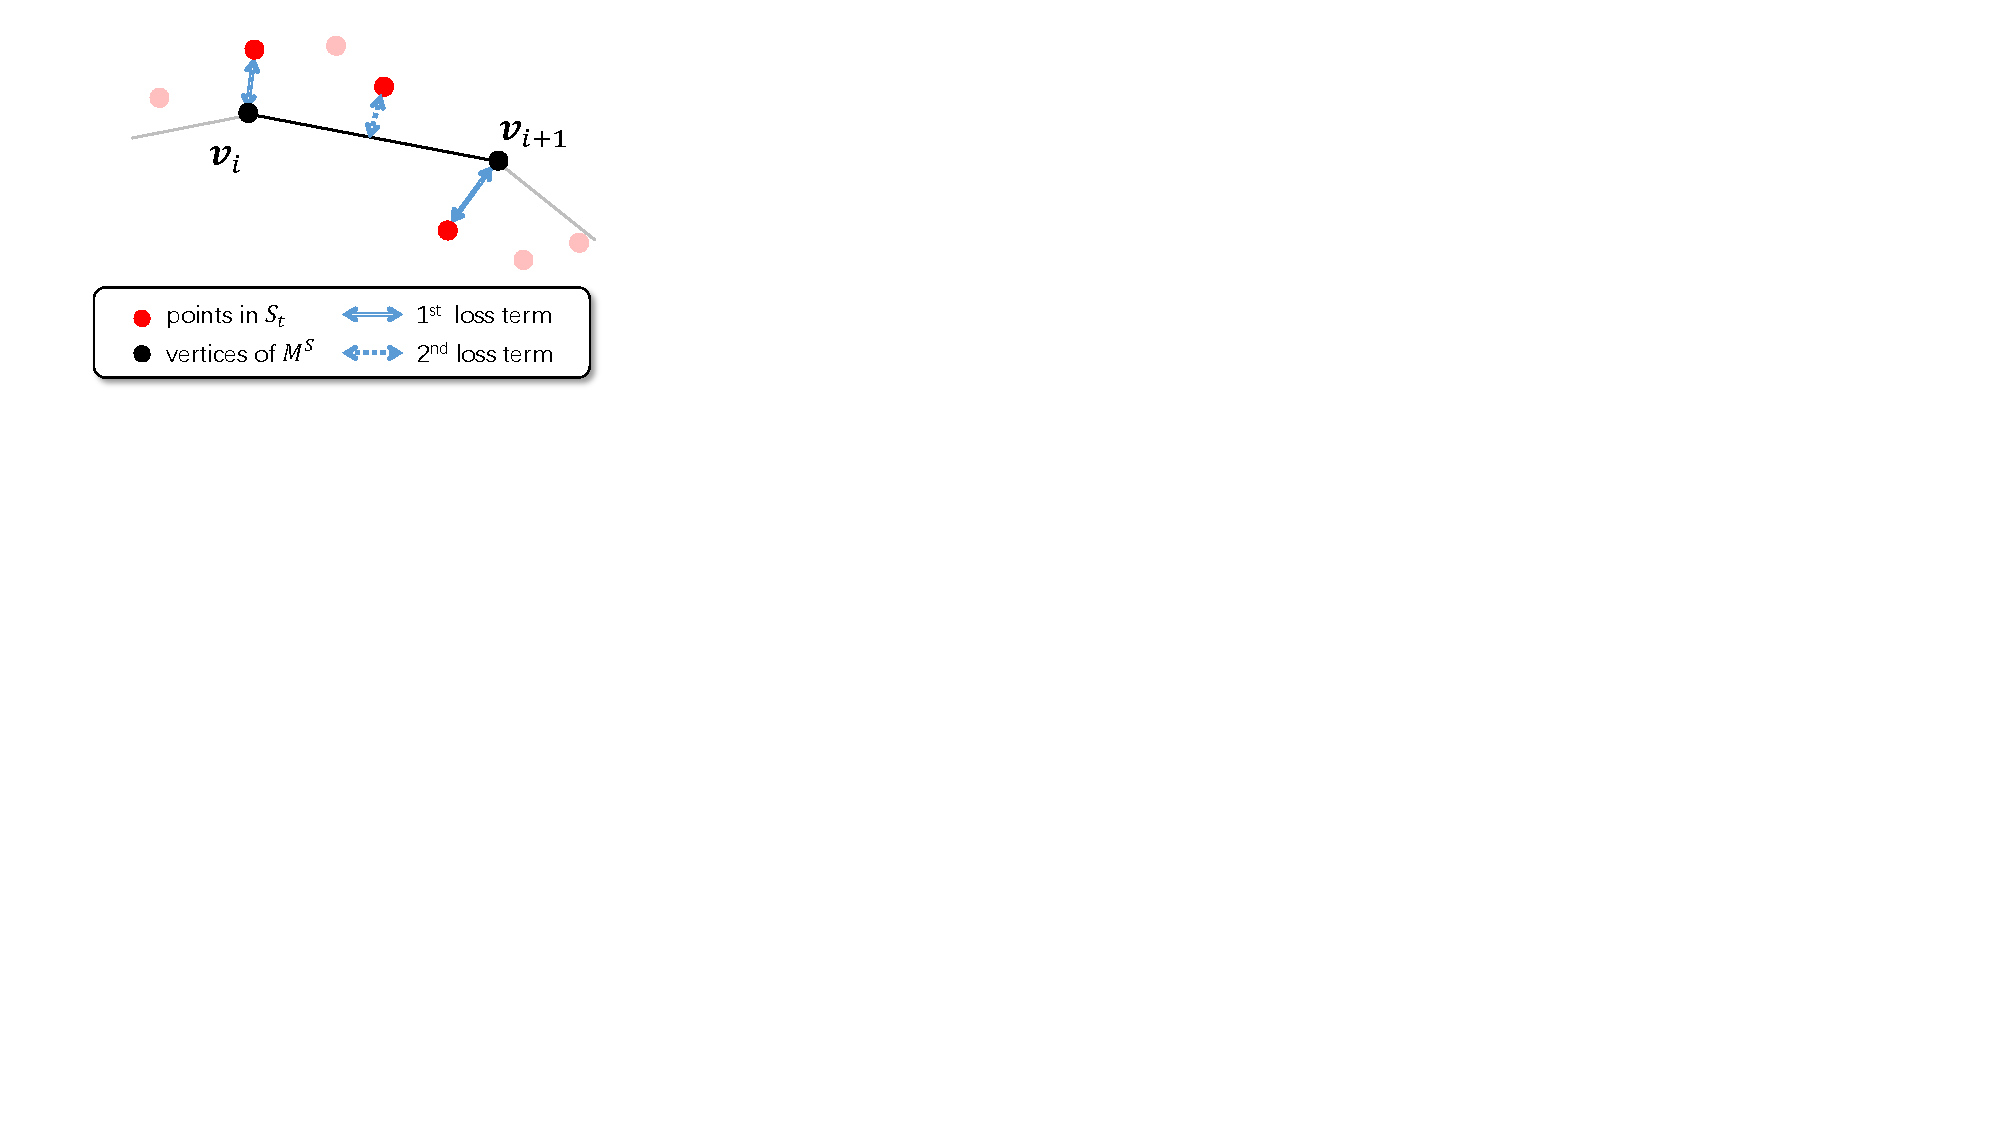
\includegraphics[width=0.5\linewidth]{chapter3/tex/figures/loss_dist.pdf}
	\end{center}
	\caption{
		\small The visualization of the distance loss $\cL_{dist}$.
	}
        % The distance loss $L_{dist}$ that is applied on vertices $v_i$, $v_{i+1}$ and the edge between them. Double arrows represent the distance penalized by the two loss terms.
	\label{ch3:fig:loss_dist}
\end{figure}

\begin{equation}
    L_{dist} = \frac{1}{|V^S|} \sum\limits_{\bv_i^S \in {V^S}} {\mathop {\min }\limits_{s \in S_t} ||s - \bv_i^S|{|^2}}  + \frac{1}{|E^S|} \sum\limits_{e_j^S \in {E^S}} {\mathop {\min }\limits_{s \in S_t} } \, dist(s,e_j^S) \, ,
\end{equation}
%
where $s$ is a sampling point in $S_t$, and $dist()$ stands for the distance of a point to a line segment. 
We denote $V^S$ the subset of vertices on the deformed airfoil profile, and $E^S$ the corresponding edges.
The first term is the sum of the distances of each point in $V^S$ to the closest point in $S_t$. The second term is the sum of the minimum distance of each edge along the airfoil profile to the closest point in $S_t$. 

\paragraph{Regularization Loss  $\cL_{reg}$.}

Minimizing $L_{dist}$ only guarantees that the decoded profile matches the target profile.  However, this only involves moving the vertices in  $\hat{V}^S$. Doing so without moving the others accordingly would produce extremely irregular and possibly overlapping computational meshes that will make CFD computations inaccurate or numerically unstable. We must therefore ensure that all vertices move accordingly to the surface vertices in order to preserve the deformed mesh quality---cells' skewness, orthogonality, aspect ratio---as well as its ability to represent the underlying physics~\cite{aa.Knupp2007}. 

\begin{figure}
    \centering
    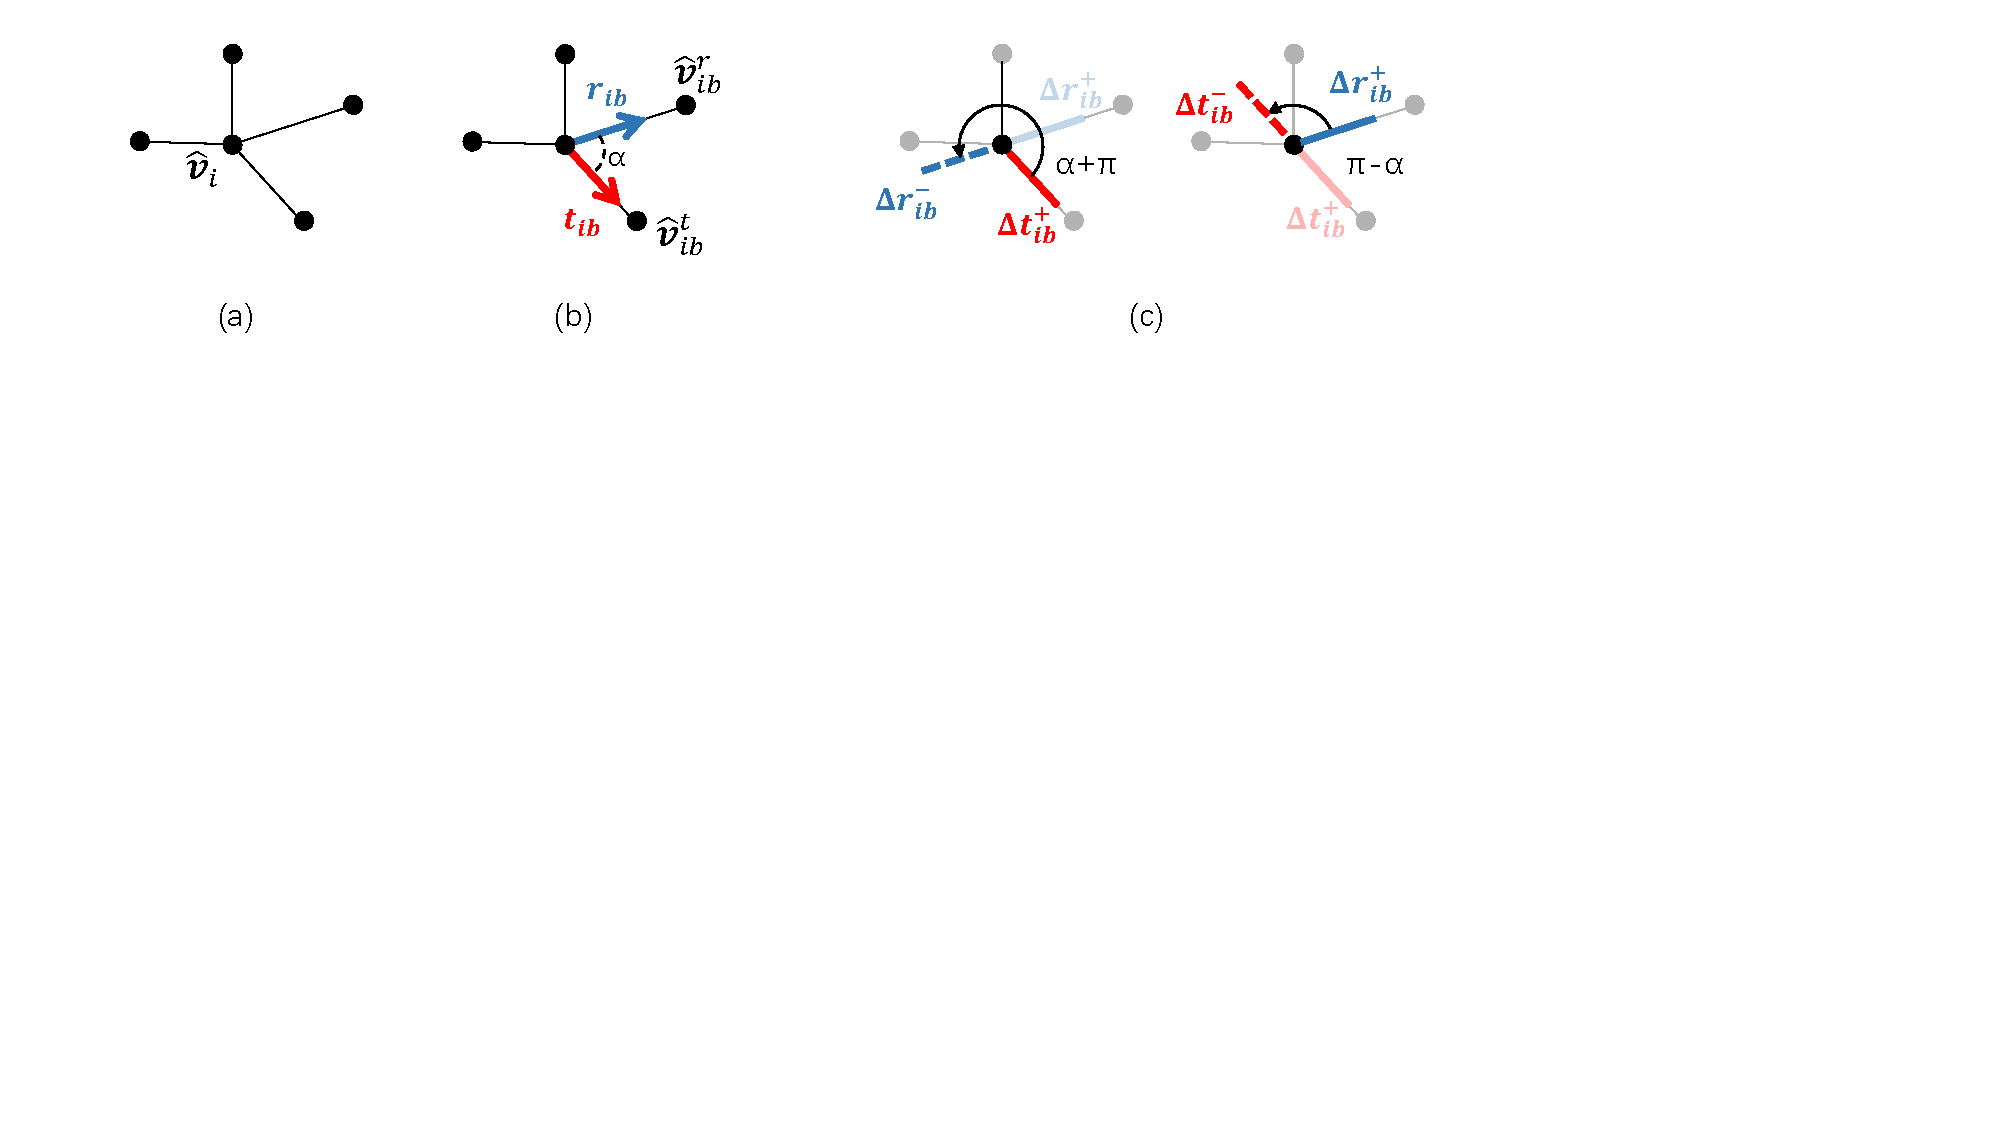
\includegraphics[width=1\linewidth]{chapter3/tex/figures/active_model_axes.pdf}
    \caption{\small The skewed coordinate systems. (a) $\hat{\bv}_i$ and its neighbors. (b) The two axes. (c) The finite difference discretization.}
    \label{ch3:fig:coords}
\end{figure}

In practice, we can assume that the template mesh $\hat{M}$ has been designed to satisfy these requirements, and we want the deformed mesh $M$ to keep on satisfying them. To this end, we introduce an energy function that quantifies the degree of distortion of $M$ with respect to $\hat{M}$. Defining $\hat{M}$ as a stationary point and then solving an extreme point finding problem yield a mesh $M$ whose local mesh structure is close to that of $\hat{M}$ so that the mesh quality priors embedded in $\hat{M}$ are preserved. To formulate this energy function, we first parameterize $\hat{M}$ using the skewed coordinate systems relying on the template mesh, as depicted by  Fig.~\ref{ch3:fig:coords}(a-b).  For each vertex $\mathbf{\hat{v}}_i$, we pair its neighboring  vertices which results in $B_i$ different two-tuples, such as $(\hat{\bv}_{i1}^r, \hat{\bv}_{i1})^t, \; (\hat{\bv}_{i2}^r, \hat{\bv}_{i2}^t), \;..., \; (\hat{\bv}_{iB_i}^r, \hat{\bv}_{iB_i}^t)$.
We pick one tuple $(\hat{\bv}_{ib}^r, \; \hat{\bv}_{ib}^t)$ and the base vectors of the coordinate system $X_{ib}$ are defined as the normalized vectors 
%
\begin{equation}
  \mathbf{r}_{ib} := \frac{{{\hat{\bv}_{ib}^r} - {\hat{\bv}_i}}}{{||{\hat{\bv}_{ib}^r} - {\hat{\bv}_i}||_2}} \; \text{ and }\; \mathbf{t}_{ib} := \frac{{{\hat{\bv}_{ib}^t} - {\hat{\bv}_i}}}{{||{\hat{\bv}_{ib}^t} - {\hat{\bv}_i}||_2}} \; .
\label{ch3:eq:new_base}
\end{equation}
%
In this base, the vertex is a function of coordinates as $\mathbf{v}(r_{ib},t_{ib})$, and vertices from the template and deformed mesh can be written as
\begin{equation}
    \left\{ 
      \begin{aligned}
          &\hat{\bv}_i(\hat{r}_{ib}, \hat{t}_{ib})= \hat{r}_{ib}\mathbf{r}_{ib}+\hat{t}_{ib}\bt_{ib} \;, \text{ for } \;  \hat{\bv}_i \in \hat{V}  \\
          &\begin{aligned}
              \bv_i(\hat{r}_{ib}, \hat{t}_{ib}) & = \hat{\bv}_i(\hat{r}_{ib}, \hat{t}_{ib}) + \mathbf{\delta\hat{v}}_i \\
              & =  \hat{r}_{ib}\mathbf{r}_{ib}+\hat{t}_{ib}\bt_{ib} + \mathbf{\delta\hat{v}}_i
          \end{aligned} 
          \;, \text{ for } \;  {\bv}_i \in V .
      \end{aligned}
    \right.
\label{ch3:eq:coords_new_base}
\end{equation}
with respect to the Cartesian origin. We attach the origin to $\hat{\bv}_i$ in Fig.\ref{ch3:fig:coords} for visualization clarity. Since we assume the template mesh is of good quality and has no zero-area cells so the collinear $(\mathbf{r}_{ib},\bt_{ib})$ is not considered.
Then by considering $M$ as a discretization of an elastic material that is framed by fixed $M^S$ and $M^{IO}$, we define the energy function at the vertex $\bv_i$ to measure the mesh distortion by summing up the squared Frobenius norm of the strain and its spatial derivative, which writes
%
\begin{align}
\mathbb{E}_{ib} &= {\left| {\left| {\nabla_{X_{ib}} \; \Delta V} \right|} \right|^2_F} + {\left| {\left| {\nabla_{X_{ib}} (\nabla_{X_{ib}} \; \Delta V)} \right|} \right|^2_F} \nonumber \\
&=  {{{\left| {\left| {{{\partial \mathbf{\delta v}_i} \over {\partial r_{ib}}}} \right|} \right|}^2} + {{\left| {\left| {{{\partial \mathbf{\delta v}_i} \over {\partial t_{ib}}}} \right|} \right|}^2} + 2{{\left| {\left| {{{{\partial ^2}\mathbf{\delta v}_i} \over {\partial r_{ib}\partial t_{ib}}}} \right|} \right|}^2} + {{\left| {\left| {{{{\partial ^2}\mathbf{\delta v}_i} \over {\partial {r^2_{ib}}}}} \right|} \right|}^2} + {{\left| {\left| {{{{\partial ^2}\mathbf{\delta v}_i} \over {\partial {t^2_{ib}}}}} \right|} \right|}^2}} \;.
\label{ch3:eq:energy}
\end{align}
%
This formulation is in the same spirit as the one used Active Surface Models (ASMs) that has been extensively studied in computer vision and computer graphics~\cite{ai.Kass1988,ai.Terzopoulos1991b,ai.Fua1996f,aa.Wickramasinghe2021}.

\begin{figure}
    \centering
    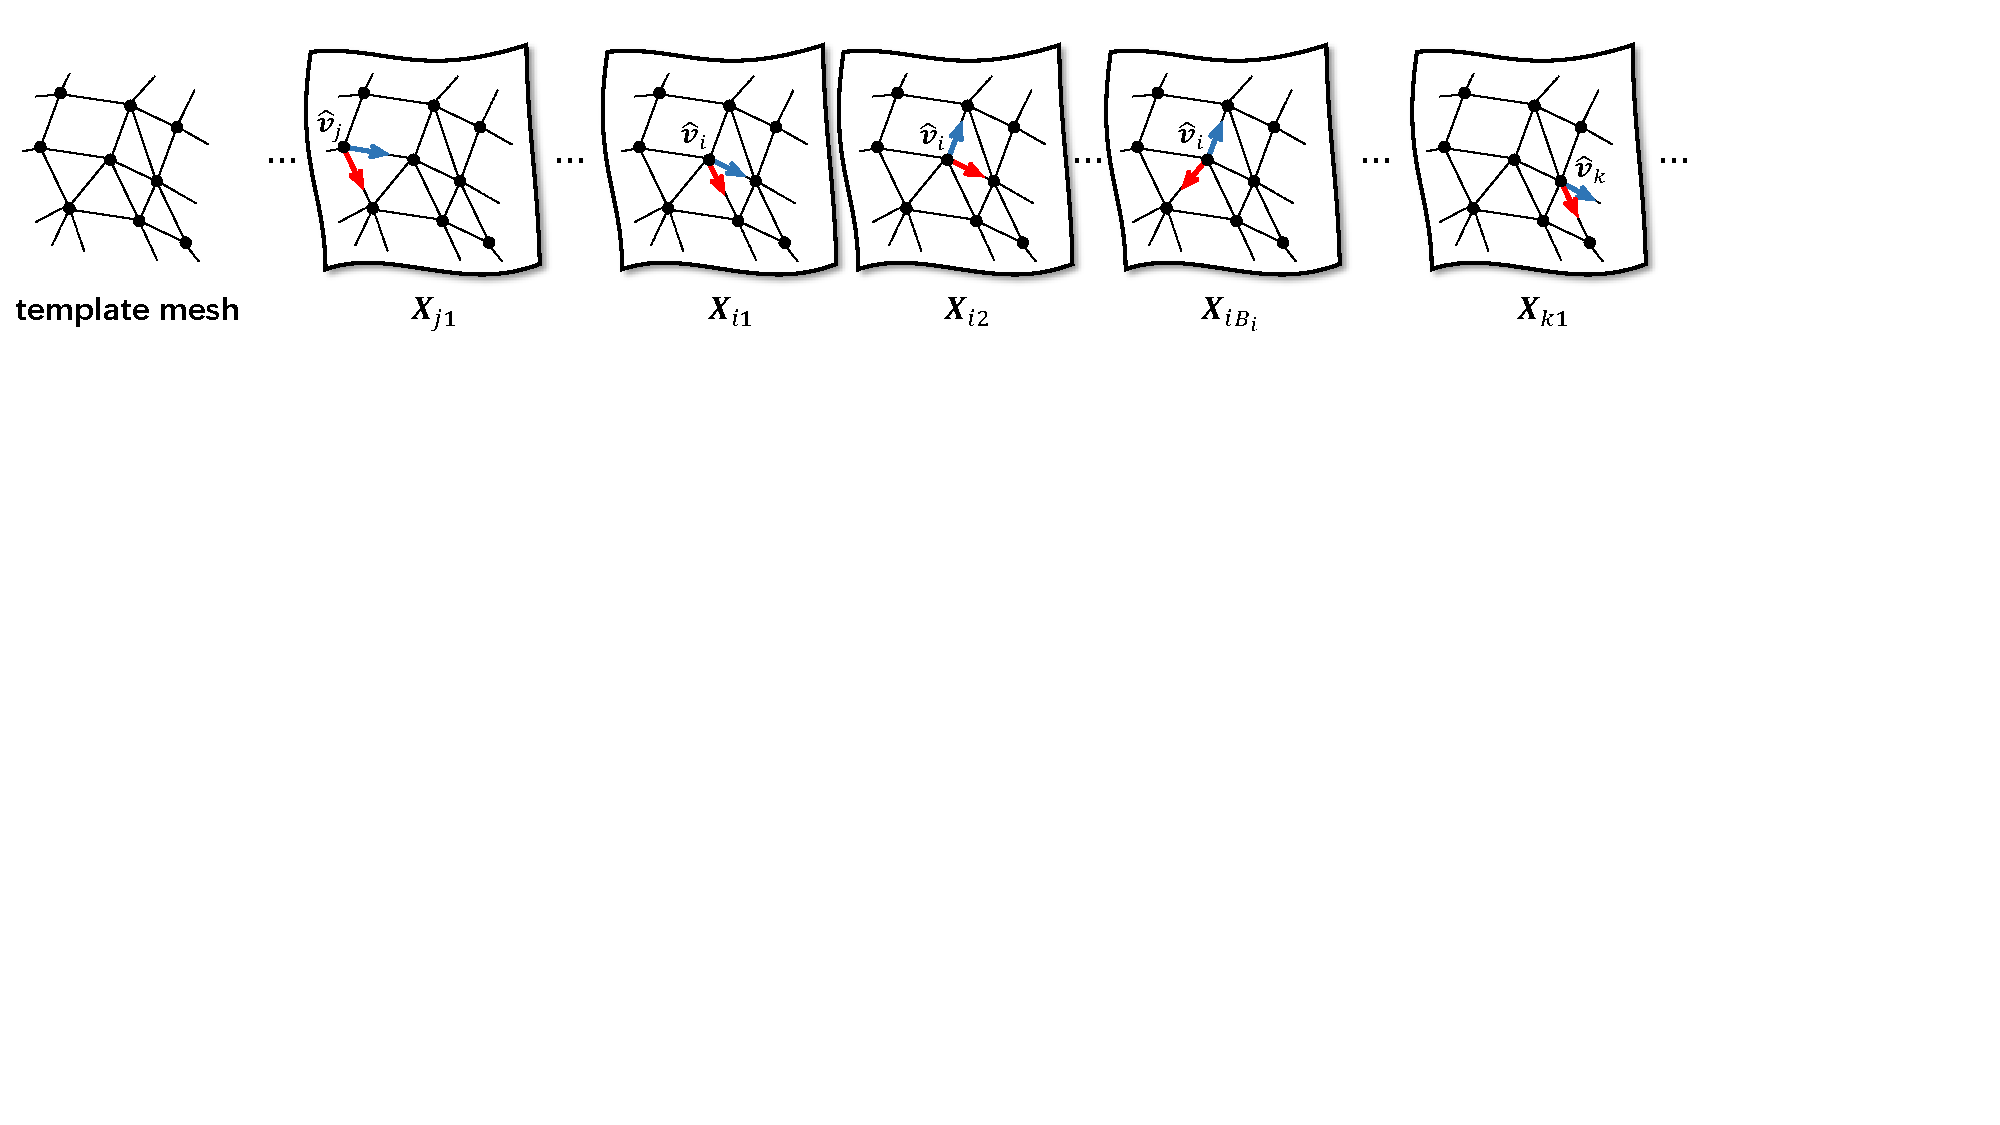
\includegraphics[width=1\linewidth]{chapter3/tex/figures/active_model_K_sum.pdf}
    \caption{\small The multiple skewed coordinate systems build on different vertex and pairs of neighbors.}
    % {\bf The template mesh and the non-rigid coordinate systems for parameterization. Each coordinate system $X$ is build on a vertex and a unique pair of neighbors. An energy function is defined for every $X$ to measure the mesh distortion locally at a certain orientation. The origins of $X$s are at the Cartesian origin. We attach it to vertices for visualization clarity} }
    \label{ch3:fig:sum_coords}
\end{figure}

To prove $\hat{M}$ is a stationary point of $\mathbb{E}_{ib}$, we look at the following formulation
%
\begin{equation}
    - \frac{\partial }{{\partial r_{ib}}}\left(\frac{{\partial \mathbf{\delta v}_i}}{{\partial r_{ib}}}\right) - \frac{\partial }{{\partial t_{ib}}}\left(\frac{{\partial \mathbf{\delta v}_i}}{{\partial t_{ib}}}\right) + 2 \frac{{{\partial ^2}}}{{\partial r_{ib}\partial t_{ib}}}\left(\frac{{{\partial ^2}\mathbf{\delta v}_i}}{{\partial r_{ib}\partial t_{ib}}}\right) + \frac{\partial }{{\partial {r_{ib}^2}}}\left(\frac{{{\partial ^2}\mathbf{\delta v}_i}}{{\partial {r_{ib}^2}}}\right) + \frac{\partial }{{\partial {t_{ib}^2}}}\left(\frac{{{\partial ^2}\mathbf{\delta v}_i}}{{\partial {t_{ib}^2}}}\right).
\end{equation}
Since $\mathbf{\delta v}_i = \bv_i - \hat{\bv}_i$ and $\partial ^2 \mathbf{\hat{v}}_i / \partial {r_{ib}^2} = \partial ^2 \mathbf{\hat{v}}_i / \partial {t_{ib}^2} = 0$ with the definition in Eq.~\ref{ch3:eq:coords_new_base}, it can be rewritten as
\begin{equation}
    F_{ib} := - \frac{\partial }{{\partial r_{ib}}}\left(\frac{{\partial \mathbf{v}_i}}{{\partial r_{ib}}}\right) - \frac{\partial }{{\partial t_{ib}}}\left(\frac{{\partial \mathbf{v}_i}}{{\partial t_{ib}}}\right) + 2  \frac{{{\partial ^2}}}{{\partial r_{ib}\partial t_{ib}}}\left(\frac{{{\partial ^2}\mathbf{v}_i}}{{\partial r_{ib}\partial t_{ib}}}\right) + \frac{\partial }{{\partial {r_{ib}^2}}}\left(\frac{{{\partial ^2}\mathbf{v}_i}}{{\partial {r_{ib}^2}}}\right) + \frac{\partial }{{\partial {t_{ib}^2}}}\left(\frac{{{\partial ^2}\mathbf{v}_i}}{{\partial {t_{ib}^2}}}\right).
    \label{ch3:eq:euler_lagrange}
\end{equation}
$F_{ib}=0$ for $\forall \, i, \, b$ when $\mathbf{v}_i = \hat{\mathbf{v}}_i$ according to the definition of $\mathbf{r}_{ib}$ and $\bt_{ib}$ in Eq.\ref{ch3:eq:coords_new_base}, which is the Euler-Lagrange equation of $\mathbb{E}_{ib}$ and is the sufficient and necessary condition of our claim. 
To regularize the computational mesh, the magnitude of $F_{ib}$ should be as small as possible to reach the stationary point of $\mathbb{E}_{ib}$. 
Since a single $\mathbb{E}_{ib}$ only describes the energy locally and at a specific orientation, we define multiple coordinates systems similarly on all vertices and with all combinations of outgoing edges
, as shown in Fig.\ref{ch3:fig:sum_coords}, as well as their corresponding energy functions and Euler-Lagrange equations.
This applies to all vertices in the computational mesh $V^{Com}$ that are not on the airfoil profile ($V^S$) nor on the in/outflow boundaries ($V^{IO}$), namely $V^{Com}=V \setminus  ({V^S \cup V^{IO}})$.
We take the regularization term $\cL_{reg}$ to be the averaged squared $F_{ib}$ as 
%
\begin{equation}
    \cL_{reg} := \frac{1}{|V^{Com}|} \sum_{i=1}^{|V^{Com}|} \frac{1}{B_i} \sum_{b=1}^{B_i} ||F_{ib}||_2^2\; ,\text{ where }\; V^{Com}=V \setminus  ({V^S \cup V^{IO}})\;.
    \label{ch3:eq:l_reg}
\end{equation}
%
Minimizing $\cL_{reg}$ yields a deformed computational mesh whose local cell structure is similar to that of $\hat{M}$. This eliminates serious issues such as overlapped facets, and desirable mesh properties embedded in $\hat{M}$, such as the cell's aspect ratio, skewness and orthogonality, are preserved as much as possible.
Using a dedicated coordinate system for every vertex and every combination of its neighbors makes $\cL_{reg}$ to work with arbitrary cell types.

\begin{figure}
    \centering
    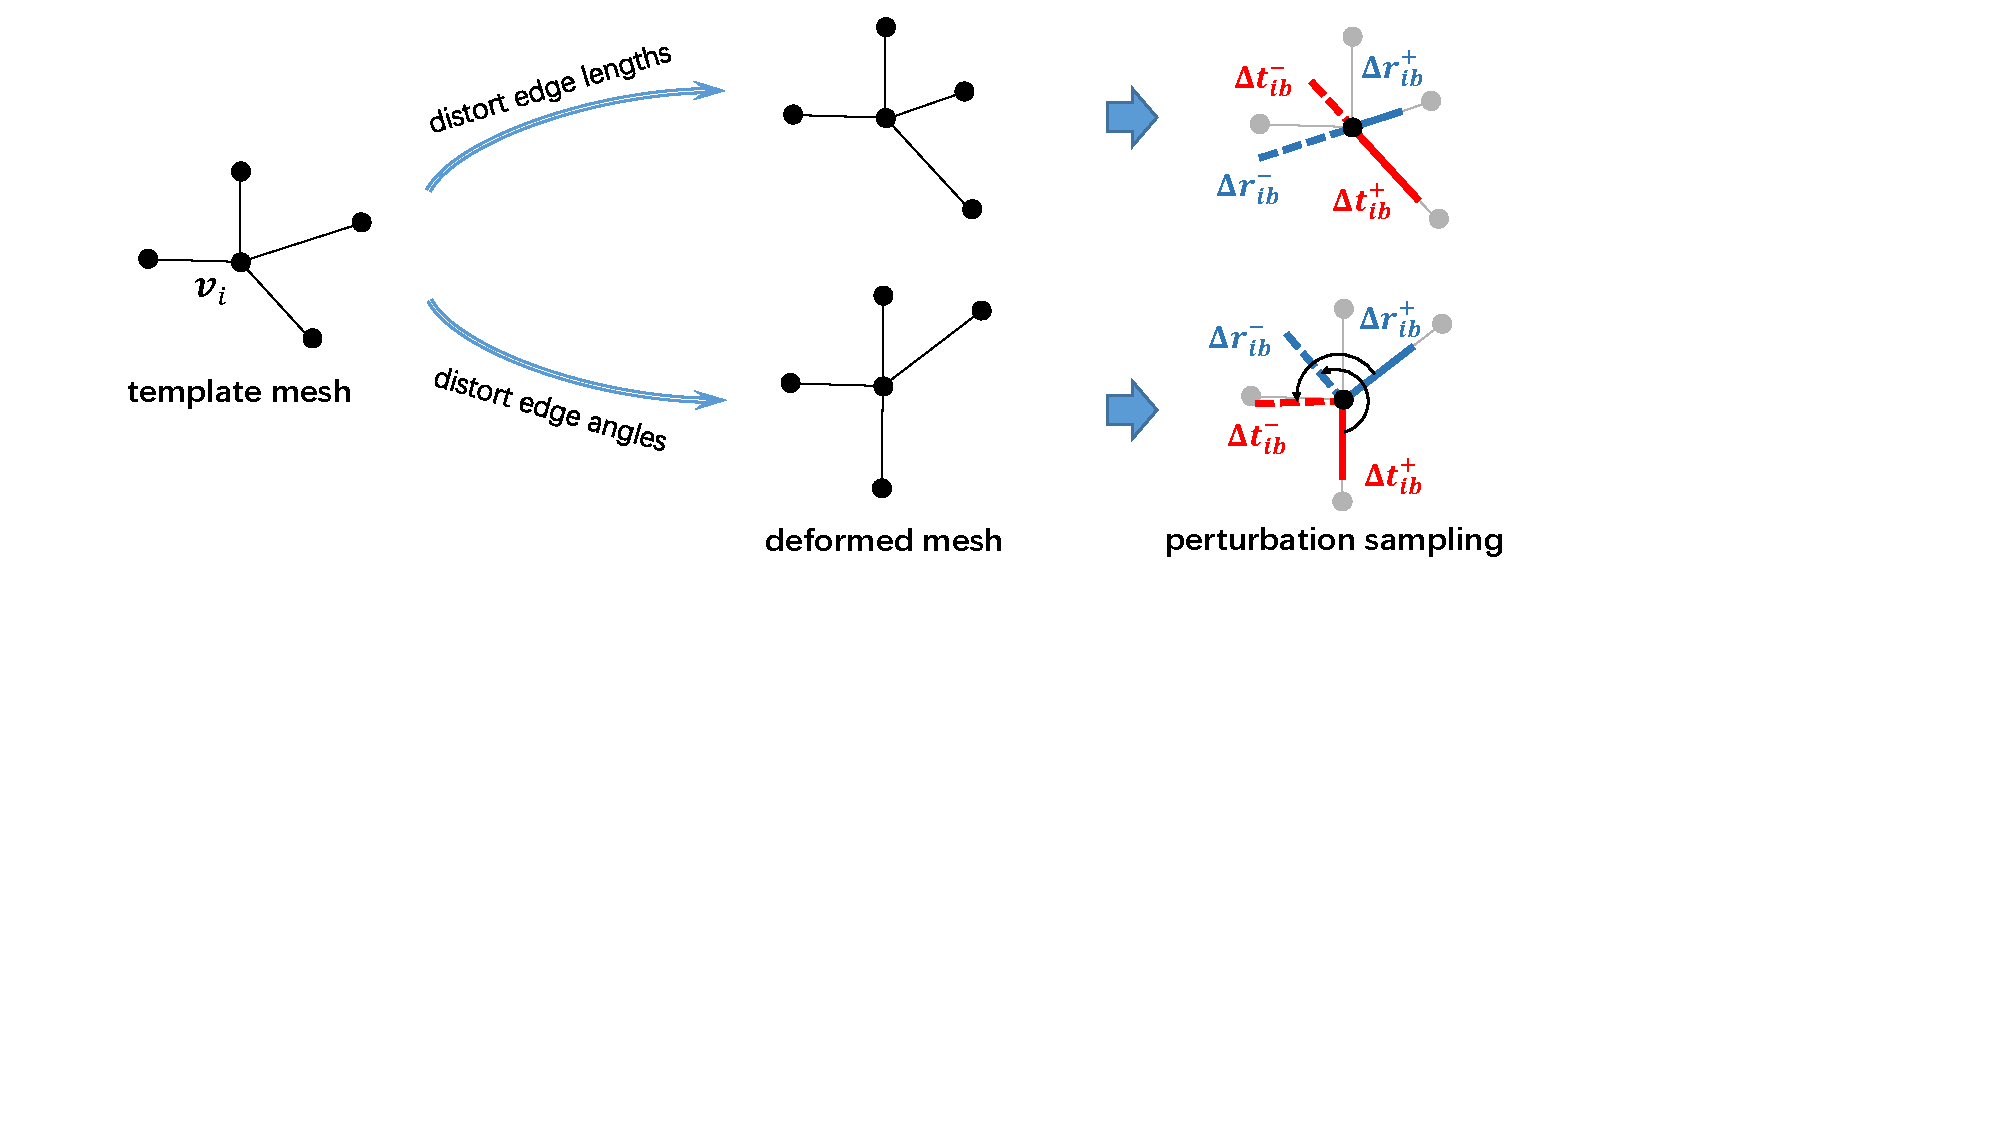
\includegraphics[width=1\linewidth]{chapter3/tex/figures/active_model_axes_distortion.pdf}
    \caption{\small {\bf Mesh distortion changes cell structures and results in nonzero $\cL_{reg}$.}
    }
    \label{ch3:fig:distort_coords}
\end{figure}

The derivatives of Eq.~\ref{ch3:eq:euler_lagrange} are estimated by finite differences. This implies computing the perturbation of vertices. As shown in Fig.\ref{ch3:fig:coords}(c), positive perturbations are sampled directly along the edges as
%
\begin{equation}
    \Delta \textbf{r}_{ib}^+ = \epsilon \frac{{{\bv_{ib}^r} - {\bv_i}}}{{||{\hat{\bv}_{ib}^r} - {\hat{\bv}_i}|{|_2}}} \;
    \text{ and } \;
    \Delta \textbf{t}_{ib}^+ = \epsilon \frac{{{\bv_{ib}^t} - {\bv_i}}}{{||{\hat{\bv}_{ib}^t} - {\hat{\bv}_i}|{|_2}}} \;,
    \label{ch3:eq:delta_r_t}
\end{equation}
%
where $\bv_{ib}^r$ and $\bv_{ib}^t$ are $\hat{\bv}_{ib}^t$ and $\hat{\bv}_{ib}^t$ after the deformation. Negative perturbations $\Delta \textbf{r}_{ib}^-$ and $\Delta \textbf{t}_{ib}^-$ are rotated from $\Delta \textbf{t}_{ib}^+$  by $\pi-\alpha$ and $\Delta \textbf{s}_{ib}^+$ by $\pi+\alpha$, respectively, where $\alpha$ is the angle between the base vectors $(\mathbf{r}_{ib}, \bt_{ib})$, i.e. $\alpha=\mathop{atan2}(|\mathbf{r}_{ib} \times \bt_{ib}| , (\mathbf{r}_{ib}\cdot \bt_{ib}))$. We keep the positive scalar $\epsilon$ small to correctly approximate the derivatives. The edge normalizers (denominators in Eq.~\ref{ch3:eq:new_base} and~\ref{ch3:eq:delta_r_t}) and the rotating angle $\alpha$ are calculated on the template mesh, and remain constant even when the mesh is distorted. 
Using the proposed coordinate system and the sampling strategy avoids complicated interpolation inside cells.
We provide additional details about the finite difference derivative  computation in Appendix\ref{ch3:sec:appendix_finite_difference} and show that they yield a valid approximation of the derivatives
%prove the correctness of this sampling strategy
in Appendix\ref{ch3:sec:appendix_sampling_proof}.
As shown in Fig.\ref{ch3:fig:distort_coords}, any type of deformations from the template mesh will leave the stationary point $\hat{M}$ since changes of edge length ratios and angles make Eq.\ref{ch3:eq:euler_lagrange} nonzero.

With this approach of approximating derivatives, each $F_{ib}$ can be written as a linear function of the position of $\bv_i$ and its neighboring vertices. Eq.\ref{ch3:eq:l_reg} can thus be rewritten as a numerical approximation with a matrix form as
\begin{equation}
    \cL_{reg} := ||K\bv||_2^2\;,
    \label{ch3:eq:discrete_euler_lagrange}
\end{equation}
where $\bv$ is the vectorized form of $V_{Com}$, where $V^{Com}=V \setminus  ({V^S \cup V^{IO}})$, and $K$ is the discretization matrix to implement the finite difference approximation.
$K$ is only dependent on the template mesh and is only generated once for the given template mesh $\hat{M}$.
Thanks to the linearity in Eq.\ref{ch3:eq:l_reg}, building multiple coordinate systems results in a single sparse $K$ matrix and does not increase the computational cost significantly.

\paragraph{Deformation Decay Loss $\cL_{dec}$.} 

We decay the vertices' motion and constrain the model to generate the minimal necessary deformation
%
\begin{equation}
    \cL_{dec} = \frac{1}{|V|} \sum_i \| \mathbf{\delta v}_i \|^2_2\;.
\end{equation}

\paragraph{Regularization Loss on Latent Space $\cL_z$.} Additionally minimizing 
%
\begin{equation}
    \cL_{z} = \frac{1}{T} \sum_t \| \bz_t \|^2_2 \; 
\end{equation}
%
amounts to assuming that the prior distribution of latent vectors is a gaussian centered around zero and helps regularize the problem. In other words, $\cL_z$ promotes smoothness of the latent space.

\subsection{Network}
\noindent \textbf{The Structure of Auto-Decoder.} 
We take the latent code $\bz$ of Eq.~\ref{ch3:eq:map} to be a 256-dimensional vector. The auto-decoder comprises 4 graph convolution layers \cite{ai.Kipf2016} and a fully connected output layer. Each graph convolution is applied with weight normalization \cite{ai.Salimans2016b} and relies on the ReLU nonlinear activation~\cite{ai.Nair2010}.
By using the term $g_\Theta(\bz;\hat{M})$, the auto-decoder concatenates the latent code at the first layer and the vertex feature in other layers with coordinates of template vertices as input at every graph convolution, and uses edge information for message passing.
Using the template vertex coordinates as inputs provide inductive bias of spatial continuity that helps the model generates smooth deformations.
The fully connected layer is applied on each vertex feature vector and predicts a 2D vertex displacement. 

\noindent \textbf{The Active Model Layer.}
At inference time, an Active Model Layer (AM layer) is used to further refine the mesh quality at a finer granularity.
The AM layer minimizes the same Eq.\ref{ch3:eq:discrete_euler_lagrange} and in an implicit post-processing approach.
Given that $K$ is not invertible, the equation can be solved iteratively as
\begin{equation}
    \lambda ({\bv^t} - {\bv^{t - 1}}) + K{\bv^t} = 0 \Rightarrow (K + \lambda I){\bv^t} = \lambda {\bv^{t - 1}}\,,
\end{equation}
where $I$ is the identity, the superscript $t$ is the iteration step and $\lambda$ is the iteration step size.
The initial state comes from the auto-decoder's direct output as $V^0=\hat{V}+\Delta V$.
Due to the large size and the sparsity of $K$, inverting $(K + \lambda I)$ precisely is impractical.
Instead, we use the Neumann series with
\begin{equation}
    {(K + \lambda I)^{ - 1}} \approx \sum\nolimits_{n = 0}^K {{{( - 1)}^n}} {\left(\frac{1}{\lambda }\right)^{n + 1}}{K^n}\,.
    \label{ch3:eq:active_model_iteration}
\end{equation}
The AM layer is necessary to eliminate minor mesh quality issue occured in auto-decoder's direct output.
We demonstrate in Sec.\ref{ch3:sec:mesh_quality} that combining the minimization of $\cL_{reg}$ and the AM layer works most effectively and efficiently.

\subsection{Training Details}

\paragraph{Training Set.}
For training purposes, we collected a set of $1100$ airfoil profiles, $T=1000$ for training and 100 for testing. We use NACA's 4-digit and 5-digit airfoils and sample random digits.  We rely on the MATLAB formulations\footnote{http://www.mathworks.com/matlabcentral/fileexchange/19915-naca-4-digit-airfoil-generator}\footnote{http://www.mathworks.com/matlabcentral/fileexchange/23241-naca-5-digit-airfoil-generator} to generate the profiles. Chord lengths are normalized to $1$, and the leading and trailing edges are fixed at $(0,0)$ and $(1,0)$, respectively. Each training profile $S_t$ is a collection of $600$ 2D points sampled on the surface of the airfoil.
Note that no topology information is in $S_t$, which enables the model to work on various type of data format, and reduces the demand for complicated data pre-processing. 

\paragraph{Template Mesh.}
%
To obtain the template mesh $\hat{M}$ of Section.~\ref{ch3:sec:formal}, we start from the NACA-0012 profile because it is the most commonly studied airfoil. We use a manually generated quadrilateral mesh~\footnote{http://www.wolfdynamics.com/tutorials.html?id=148} as the default template mesh. It contains $116,240$ vertices and $230,920$ faces. The computational boundaries are at least $14$ chords away from the airfoil. The mesh is extruded and there is only one cell along the $z$ axis. As shown in Fig.~\ref{ch3:fig:exp_default_template}, we reduce the required amount of computation by fixing some of the exterior vertices and only allowing those closer to the profile to move.

Unless otherwise specified, the quadrilateral mesh in mention is used in experiments by default, denoted as TM-A. The proposed model also works well on other types of meshes, even without any adaptation on the network after training, which will be further discussed in Sec.\ref{ch3:sec:discussion_different_mesh}.

\paragraph{Implementation Details.}

We use the Pytorch~\cite{ai.Paszke2019} library for implementation. During training, we used the Adam optimizer \cite{ai.Kingma2015b} to solve Eq.~\ref{ch3:eq:autoenc} with a learning rate of $5\times 10^{-4}$ for the decoder weights and $10^{-3}$ for the latent codes. The training batch size was $5$ and we ran $20$ training epochs. We took the weights of Eq.~\ref{ch3:eq:totLoss} to be $w_{dist}=3\times 10^3, w_{reg}=10^3, w_{dec} = 10^{-3}, w_{z}=10^{-4}$.
At inference time, the decoder remains fixed while the latent code for a reference geometry is initialized with Gaussian noise. It is then optimized with $800$ gradient descent steps and a learning rate of $5\times 10^{-4}$.